%%%%%%%%%%%%%%%%%%%%%%%%%%%%%%%%%%%%%%%%%%%%%%%%%%%%%%%%%%%%%%%%%%%%%%%%%%%%
% Broad Impact 
%%%%%%%%%%%%%%%%%%%%%%%%%%%%%%%%%%%%%%%%%%%%%%%%%%%%%%%%%%%%%%%%%%%%%%%%%%%%

\chapter{Broad Impact: United Nations SDGs}
\label{chapter:Broad_Impact}
%In this chapter, you need to discuss the broad impact of your FYP. You need to explain briefly how does your project meet or satisfy any of the 17 UN SDGs (please check the power point available on Moodle about the UN SDGs).

\noindent The impact of SoleMate goes beyond its technical implementation. This project addresses various healthcare and innovation issues that are associated with multiple Sustainable Development Goals (SDGs) established by the United Nations (UN), shown in Fig. ~\ref{fig:sdg}. SoleMate was developed as a wearable health-monitoring platform that integrates plantar-pressure sensing, PPG-based measurements, swelling detection, machine-learning analysis, and mobile-application support within a unified system. It aims to implement continuous gait and cardiovascular monitoring when standard healthcare procedures are insufficient. Based on that, this project is relevant to SDG 3, Good Health and Well-Being, SDG 9, Industry, Innovation and Infrastructure, SDG 10, Reduced Inequalities, and indirectly SDG 11, Sustainable Cities and Communities \cite{un_goals}.\\

\begin{figure}[htbp]
    \centering
    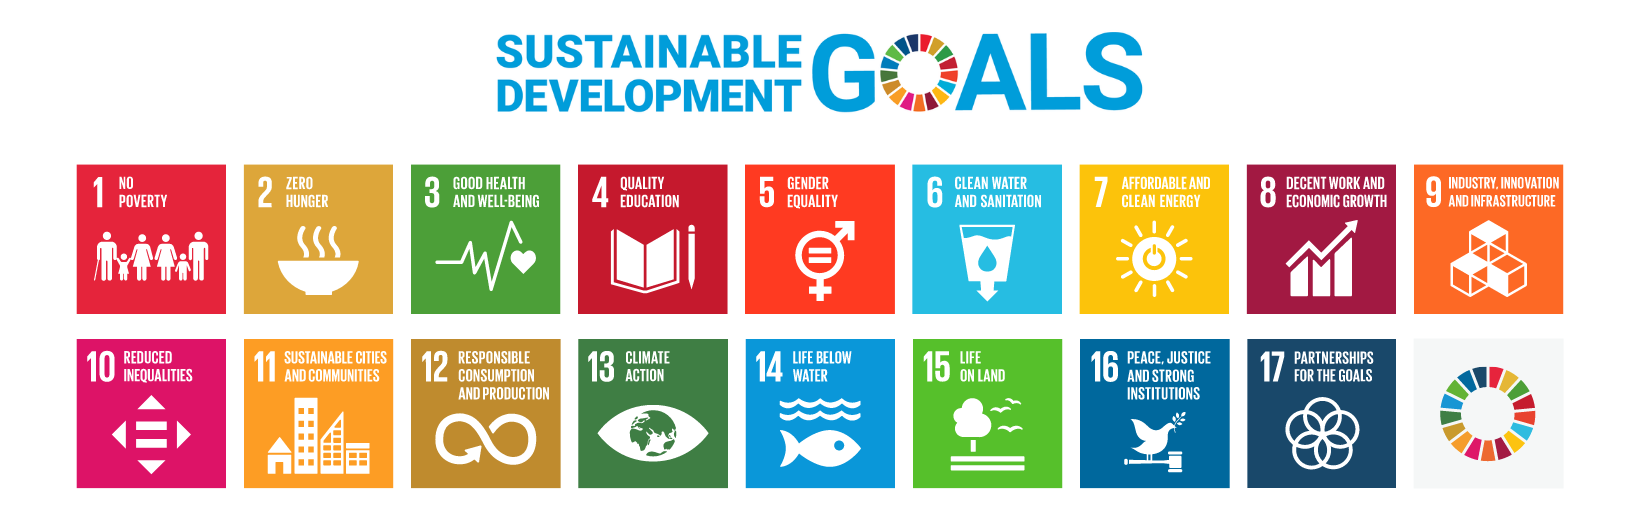
\includegraphics[width=\linewidth]{FYP_Template_Spring/Figures/sdg.png}
    \caption{Sustainable Development Goals by the United Nations.}
    \label{fig:sdg}
\end{figure}

\section{SDG 3: Good Health and Well-Being}
The project's greatest impact falls under SDG 3: Good Health and Well-Being, shown in Fig. ~\ref{fig:sdg3}. SoleMate is designed to monitor physiological and biomechanical indicators continuously. This data may reveal early signs of health deterioration. By integrating pressure sensors for plantar pressure readings, PPG sensors for heart rate and oxygen saturation measurements, and flex sensors for ankle swelling detection, the system can collect various indicators related to various health conditions.For neurological and cardiovascular conditions, continuous monitoring becomes crucial because minor alterations in health status can develop gradually and remain undetected until the next clinical visit. SoleMate addresses this limitation by enabling continuous wearable monitoring instead of relying solely on isolated testing in episodic clinical visits. This broadens the role of technology in preventive care, follow-up, and health monitoring. Therefore, the project clearly supports SDG 3 by contributing to improved health monitoring, earlier diagnosis, and better long-term well-being.\\

\begin{figure}[htbp]
    \centering
    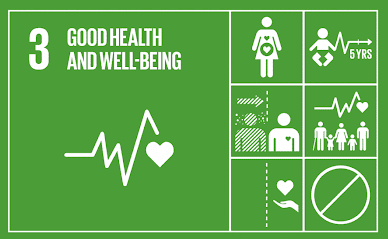
\includegraphics[width=\linewidth]{FYP_Template_Spring//Figures/SDG3.png}
    \caption{United Nations Sustainable Development Goal 3: Good Health and Well-Being.}
    \label{fig:sdg3}
\end{figure}

\section{SDG 9: Industry, Innovation and Infrastructure}
The project aligns with SDG 9: Industry, Innovation, and Infrastructure, shown in Fig. ~\ref{fig:sdg9}. SoleMate represents the development of an advanced biomedical engineering system, which integrates hardware, software, artificial intelligence, and mobile communications. Since SoleMate incorporates the development of a custom biomedical sensing system, real-time heatmap visualization, and machine-learning-based data-driven classification, it illustrates a high level of engineering innovation. These elements make the project a strong example of SDG 9 applied to real societal needs. SoleMate contributes to SDG 9 by supporting technological advancement, encouraging locally relevant innovation, and demonstrating how modern engineering tools can be used to create new healthcare-oriented infrastructure and smart monitoring systems.\\

\begin{figure}[htbp]
    \centering
    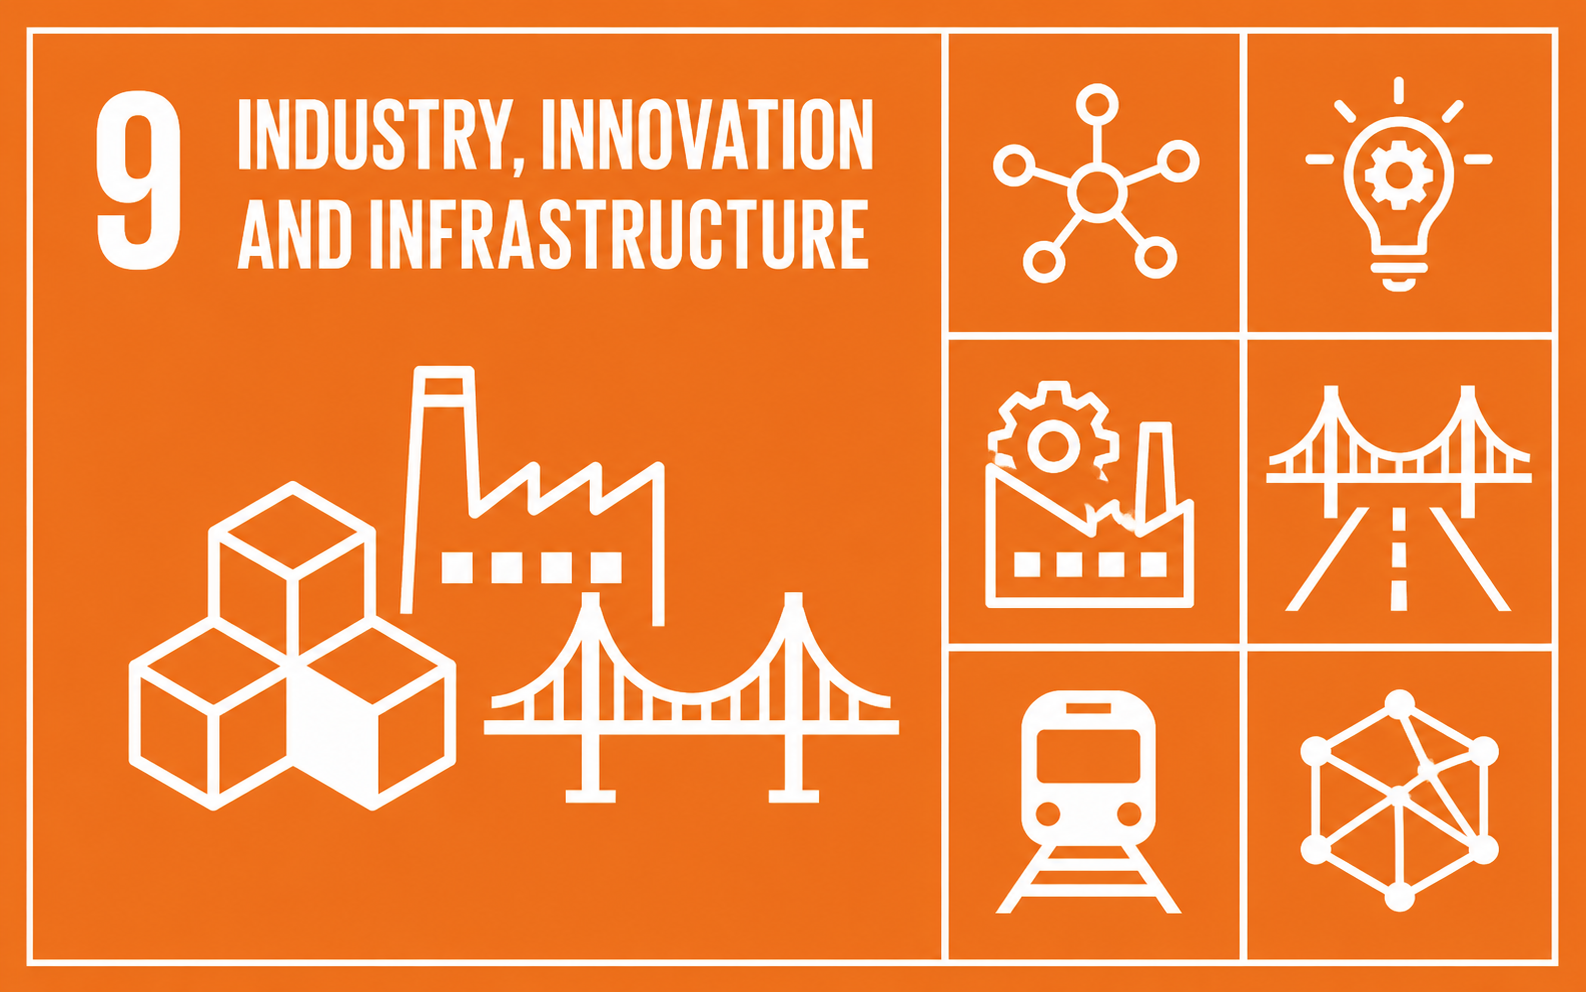
\includegraphics[width=\linewidth]{FYP_Template_Spring/Figures/SDG9.png}
    \caption{United Nations Sustainable Development Goal 9: Industry, Innovation and Infrastructure}
    \label{fig:sdg9}
\end{figure}

\section{SDG 10: Reduced Inequalities}
Although not as direct as previous SDGs, this project falls under SDG 10: Reduced Inequalities, shown in Fig. ~\ref{fig:sdg10}. SoleMate does not reduce health inequalities by solving structural problems in the healthcare industry. Instead, this project, through developing a wearable technology, could decrease the number of clinical visits, which could reduce the economic burden of neurological and cardiovascular diseases. SoleMate could also complement existing clinic-based gait analysis systems. As many diagnostic devices remain costly and out of reach for many neurological and cardiovascular patients, SoleMate could contribute to increasing accessibility and equality in healthcare. \\

The importance of this contribution is due to the growing demand for cost-effective and readily available diagnostic devices within the healthcare sector. SoleMate may also serve underprivileged communities, such as those in Lebanon. The connection between SoleMate and SDG 10 can be seen as a contribution towards the objective indirectly, through the enhancement of accessibility, rather than as a means of directly addressing the issue at hand. \\

\begin{figure}[htbp]
    \centering
    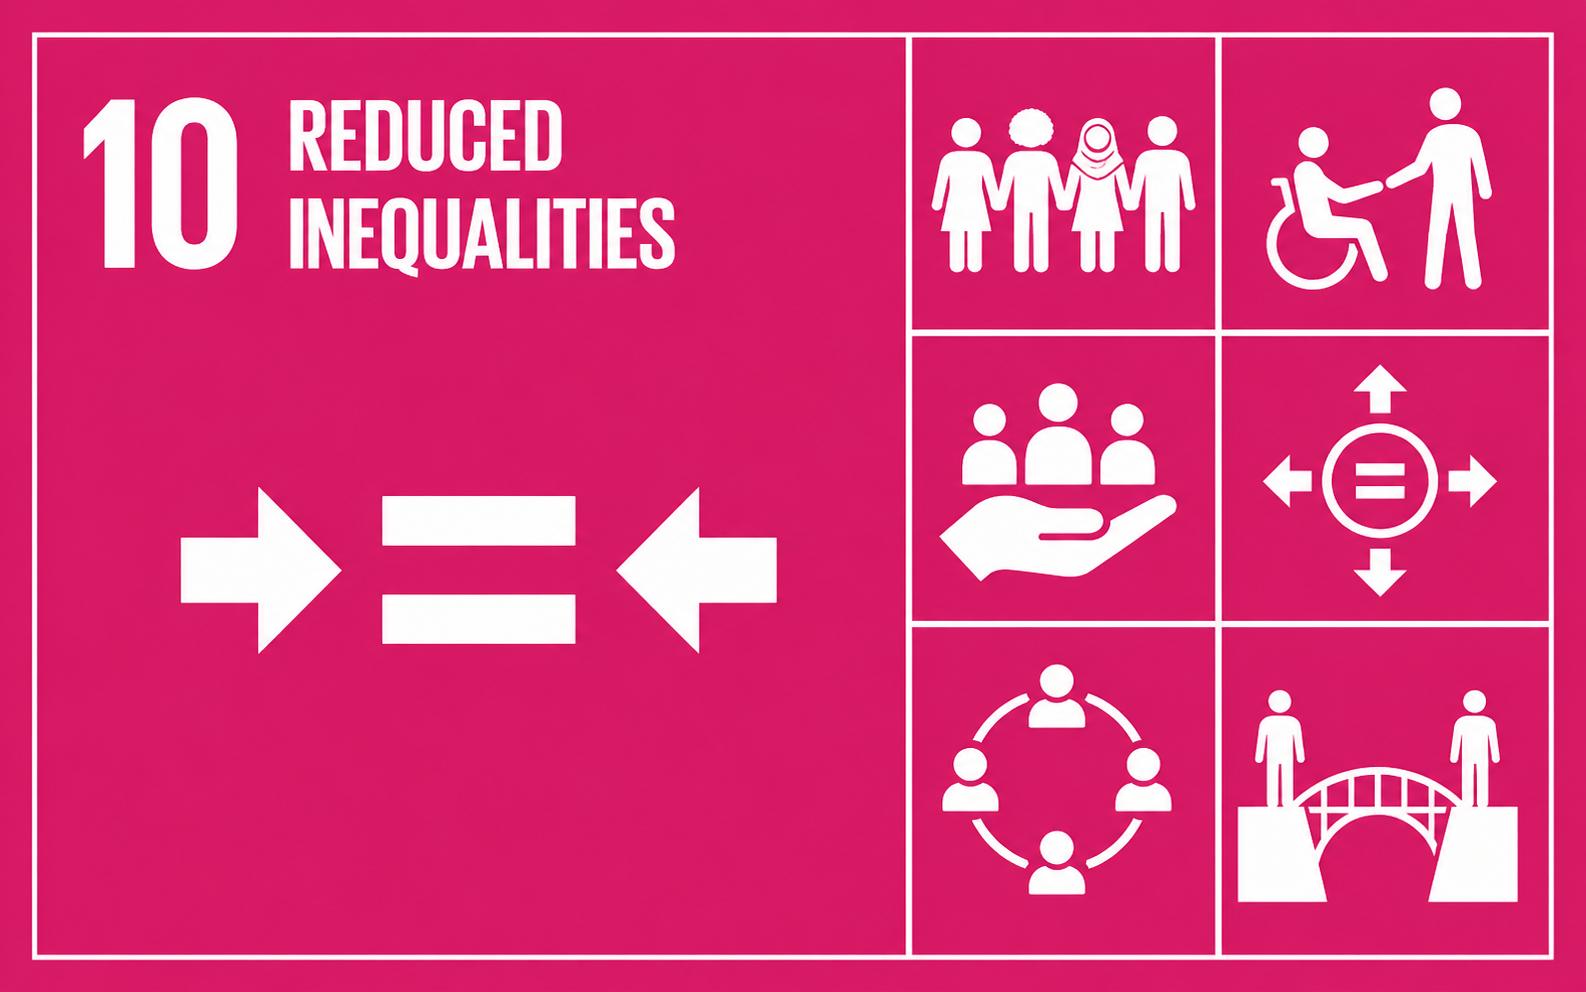
\includegraphics[width=\linewidth]{FYP_Template_Spring/Figures/SDG10.png}
    \caption{United Nations Sustainable Development Goal 10: Industry, Innovation and Infrastructure}
    \label{fig:sdg10}
\end{figure}

\section{SDG 11: Sustainable Cities and Communities}
SoleMate contributes to SDG 11: Sustainable Cities and Communities, shown in Fig. ~\ref{fig:sdg11}, by supporting the transition from centralized clinic-based healthcare to decentralized community-based monitoring. By enabling patients to continuously monitor their health from the comfort of their own home, the system reduces the load on hospitals. Instead of visiting the hospital regularly, SoleMate tracks patient data and notifies clinicians of significant findings remotely through the accompanying app.\\

This approach contributes to a more efficient healthcare system by optimizing the use of medical resources. By decreasing hospital visits, SoleMate decreases the frequency of transportation to healthcare facilities. This helps lower the economic burden on patients, while also contributing to a more sustainable urban environment.\\

\begin{figure}[htbp]
    \centering
    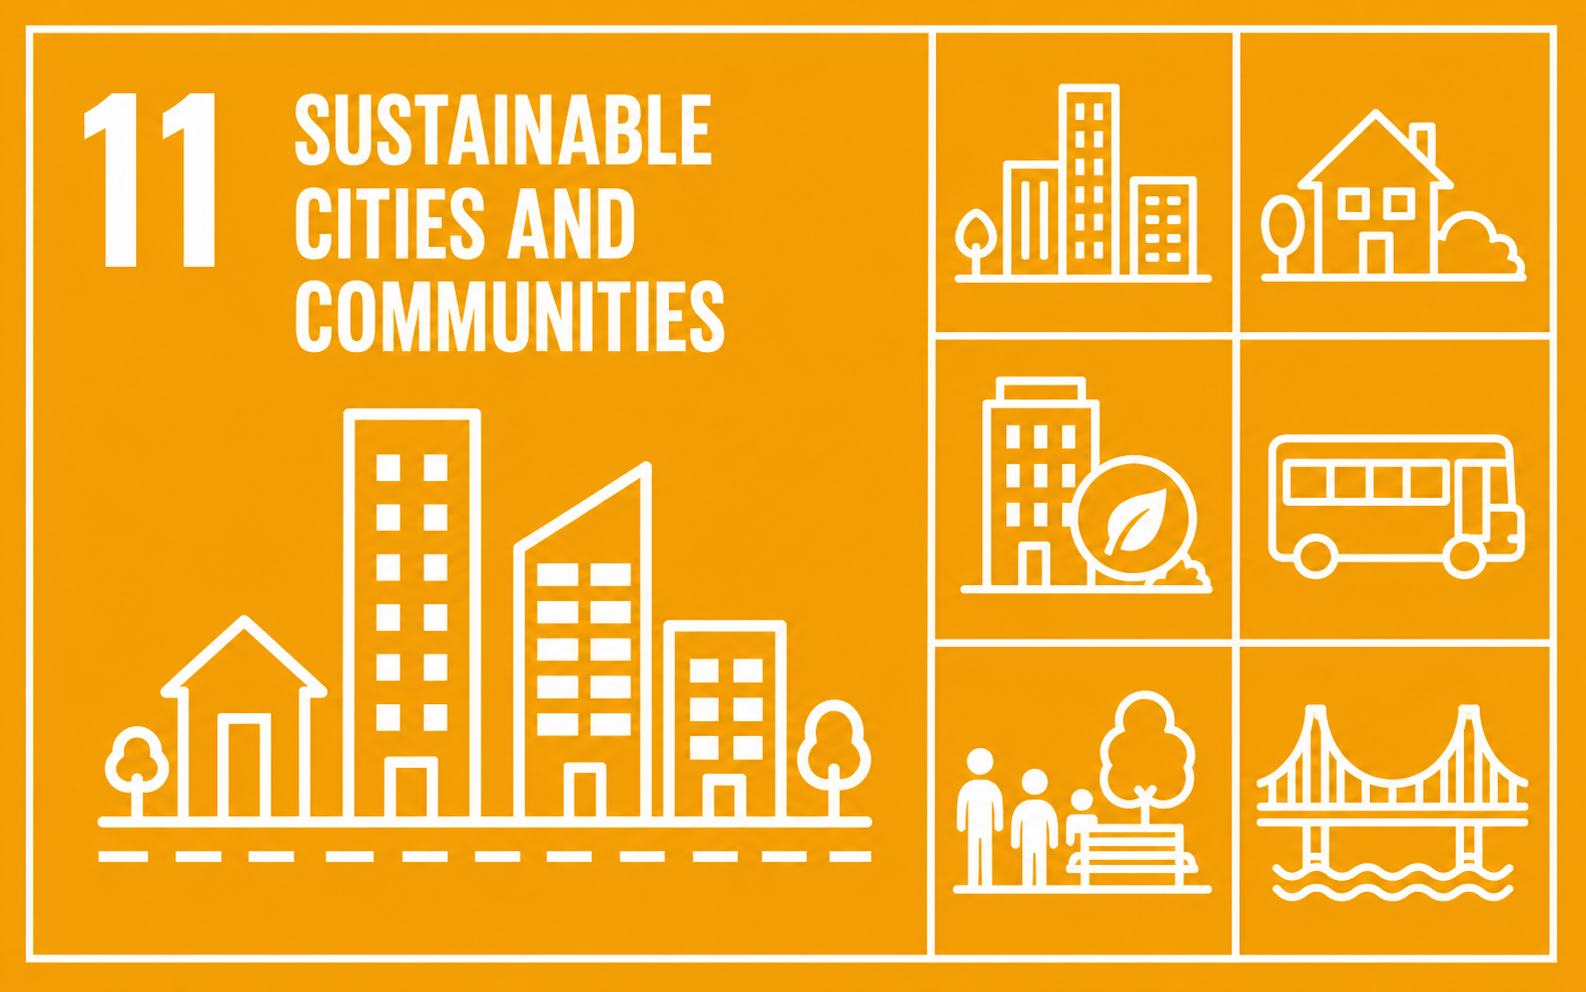
\includegraphics[width=\linewidth]{FYP_Template_Spring/Figures/SDG11.png}
    \caption{United Nations Sustainable Development Goals 11: Sustainable Cities and Communities}
    \label{fig:sdg11}
\end{figure}

\newpage
In general, SoleMate demonstrates that engineering projects can extend beyond their technical functions by providing meaningful contributions to healthcare and society, as illustrated in Fig. ~\ref{fig:sdgprj}. In particular, the system enhances individual well-being by enabling continuous health monitoring, which supports the early detection of potential medical conditions and reduces the risk of undetected health deterioration. \\

SoleMate also reflects a multidisciplinary approach to design by integrating multiple technological innovations under one unified system: multi-sensors, AI, and mobile devices and applications. This integration highlights how modern engineering solutions can address real-world healthcare challenges while contributing to broader societal goals. \\

\begin{figure}[htbp]
    \centering
    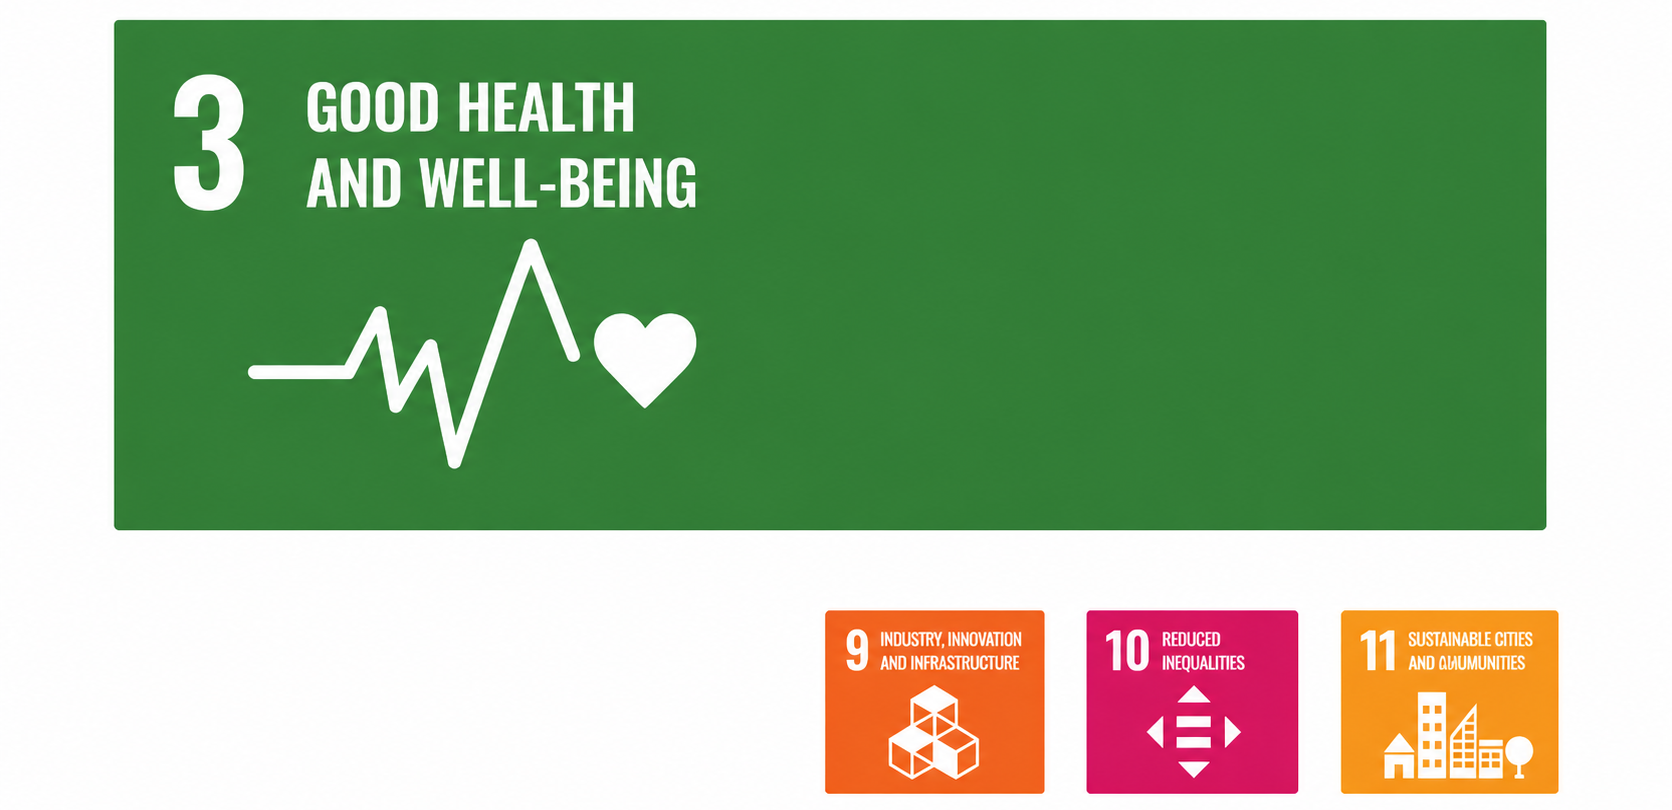
\includegraphics[width=\linewidth]{FYP_Template_Spring/Figures/SDG_Proj.png}
    \caption{Sustainable Development Goals addressed by the SoleMate project}
    \label{fig:sdgprj}
\end{figure}


